\chapter{Resultados numéricos}

Para estudiar la respuesta electromagnética (EM) de una monocapa de nanopartículas (NPs) inmersa en un medio dieléctrico, denominado matriz, y soportada sobre un sustrato dieléctrico, se emplea el formalismo del modelo de esparcimiento coherente (Coherent Scattering Model, CSM) para calcular la reflectancia $R$ y transmistancia $T$ del sistema \cite{reyes2018analytical}. El CSM proporciona expresiones analíticas de los coeficientes de amplitud de reflexión $r$ y transmisión $t$ de la monocapa cuando está suspendida en el espacio libre (Free Stanting Monolayer, FSM) [Ecs. \eqref{eqs:rtcoh}], y para el sistema matriz-monocapa-sustrato tanto en incidencia externa [Ecs. \eqref{eqs:rtCSMext}] como interna, o bien en una configuración de reflexión total atenuada \index{Reflexión total!atenuada} (Attenuated Total Reflection, ATR) [Ecs. \eqref{eqs:rtCSMATR}]. En la primera sección de este capítulo se calcula la respuesta EM de una moncapa de NPs esféricas considerando que la función dieléctrica de las NPs que conforman la monocapa está dada por el modelo de Drude-Sommerfeld [Ec. \eqref{eq:Drude}], que depende de sólo dos parámetros: la frecuencia de plasma $\omega_p$, que sintoniza las resonancias plasmónicas de superficie (Surface Plasmon Resonances, SPRs), y la constante fenomenológica de amortiguamiento $\gamma$, que ajusta el ancho de cada SPR. En caso de identificar en el cálculo de la refectancia y transmitancia de una monocapa de NPs excitaciones distintas a las  SPRs de partículas individuales (Single Particles SPR, SP-SPRs), como el \emph{modo guiado} reportado en \cite{kabashin2009plasmonic} y \cite{danilov2018ultra}, también denominado resonancia de red de plasmón de superfice (Surface Plasmon Lattice Resonance, SPLR), la elección de $\omega_p$ y $\gamma$ evita el traslape entre ambas excitaciones y facilita la identificación de cada modo. En la segunda sección se emplean las correcciones por tamaño para partículas esféricas de las funciones dieléctricas del oro y de la plata, para identificar si un modo semejante al modo guiado se encuentra en monocapas formadas con NPs de materiales reales, así como las  características de la monocapa para que pueda ser empleada en el biosensado.

\section{Resultados con el modelo de Drude-Sommerfeld}
\label{section:Drude}


 En la primera subsección se analiza la reflectancia de una FSM empleando el modelo de Drude-Sommerfled con parámetros $\hbar\omega_p = 4.3$ eV y  $\hbar\gamma = 0.15$ eV [ver Fig. \ref{sfig:Drude4eV}], y comparando la respuesta EM de la monocapa con la de una partícula individual. En la segunda subsección se estudia la reflectancia de una monocapa soportada en configuración de reflexión interna atenuada, ver Fig. \ref{sfig:ATR}, empleando el modelo de Drude-Sommerfeld en un primer caso con los parámetros  $\hbar\omega_p = 4.3$ eV y  $\hbar\gamma = 0.15$ eV, y posteriormente con $\hbar\omega_p = 10$ eV y $\hbar\gamma = 0.15$ eV [ver Fig. \ref{sfig:Drude10eV}] para modificar la longitud de onda de las SP-SPRs; ulteriormente se calcula la reflectancia de la monocapa considerando  variaciones en la fracción de cubierta $\Theta$ y el radio $a$ de las NPs, parámetros que modifican las proporciones del sistema, tales como la distancia promedio entre las NPs, y la cantidad de electrones libres sobre la monocapa. Adicional al cálculo de la reflectancia, se calculó la transmitancia de la monocapa para las dos funciones dieléctricas, con $\hbar\omega_p =4.3$ eV y $\hbar\omega_p =10$ eV, para corroborar que los modos distintos a las SP-SPRs tienen un comportamiento semejante a un modo guiado. 
	
	\subsection{Reflectancia de una monocapa suspendida en aire}
	\label{ssection:DrudeFSM}
	
	
Para el cálculo de la reflectancia mediante el CSM de una FSM suspendida en una matriz con $n_m=1.33$, modelando al agua en el espectro visible \cite{INDREF}. Se empleó la Ec.  \eqref{eq:R} con el coeficiente de amplitud de reflexión coherente $r_{coh}$ [Ec.  \eqref{seq:rcoh}].  En la Fig.  \ref{fig:R-FSM} se muestran los resultados de la reflectancia $R$ en función del ángulo de incidencia $\theta_i$ y tanto de la longitud de onda $\lambda$ del haz incidente (escala inferior), como de la energía del haz incidente en unidades de $\hbar\omega = h c /\lambda$ (escala superior).  La frecuencia de plasma empleada para la función dieléctrica tipo Drude fue $\hbar\omega_p = 4. 3$ eV y la constante fenomenológica de amortiguamiento $\hbar\gamma = 0. 15$ eV (que corresponden a $288. 5$ nm  y $8,270$ nm, respectivamente). Se consideraron NPs de radio $a=30$ nm y fracciones de cubierta $\Theta$: $0. 05$, $0. 1$, $0. 2$, $0. 3$ y $0. 4$. En el renglón superior de la Fig. \ref{fig:R-FSM}, gráficas de $\mathbf{i)}$ a $\mathbf{v)}$, se muestra la reflectancia para polarización \emph{p}, mientras que en el renglón inferior se presentan las gráficas para polarización \emph{s}, $\mathbf{vi)}$ -- $\mathbf{x)}$. La línea punteada vertical verde  en $\lambda \approx 658$ nm corresponde a la SP-SPR dipolar ($\ell = 1$), mientras que la línea vertical rosa punteada en $\lambda \approx 561$ nm corresponde a la excitación del modo cuadrupolar ($\ell=2$).
					
	\begin{figure}[h!]\centering
	\begin{tikzpicture}
\node[inner sep=0pt] (graf) at (-.15,0){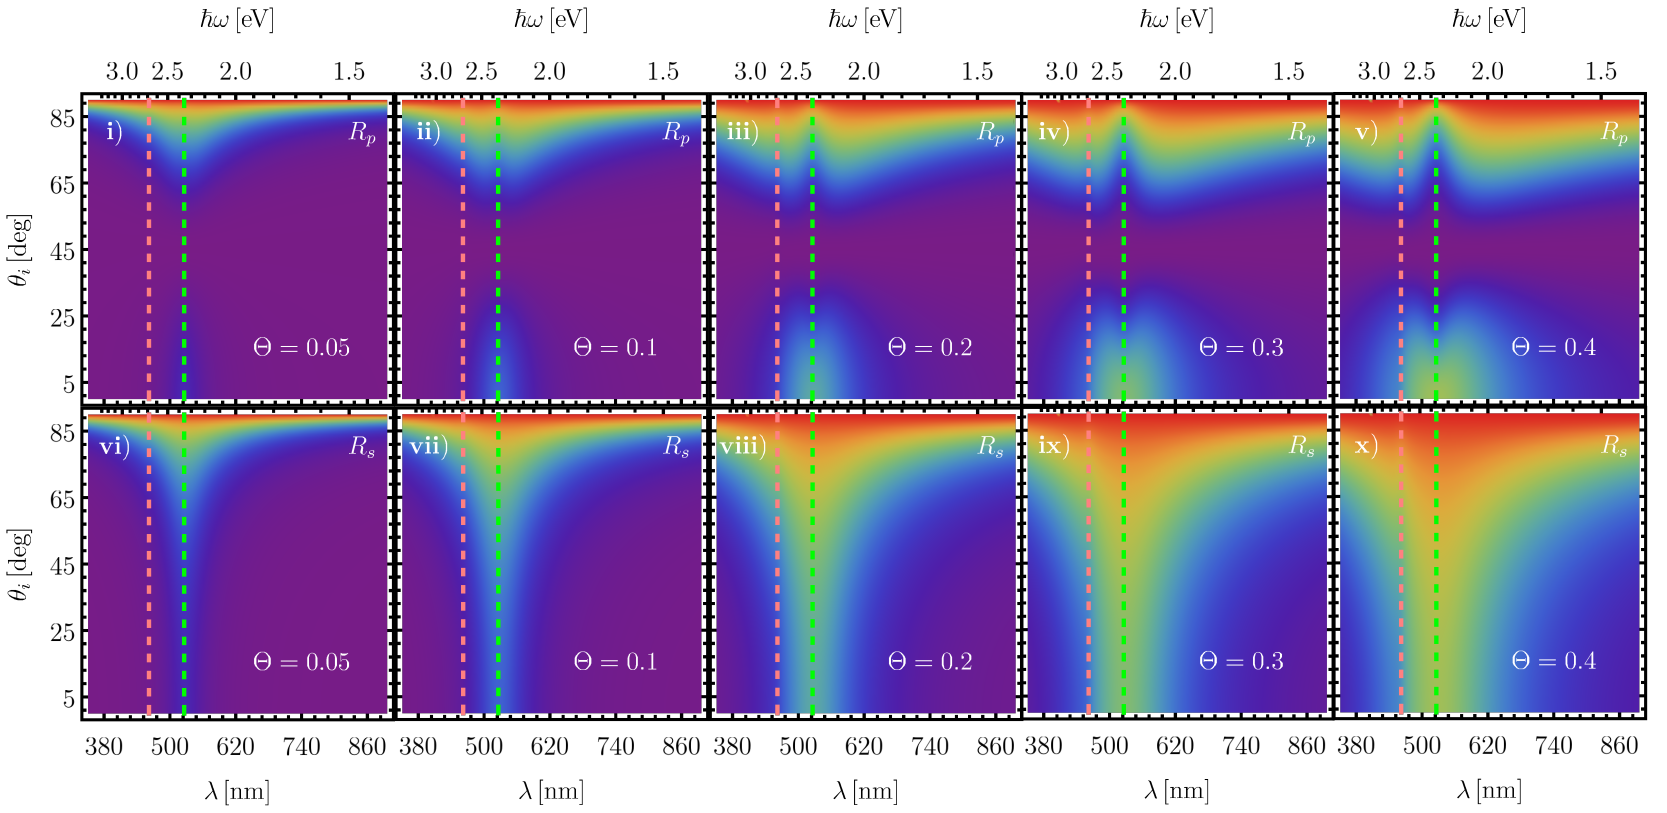
\includegraphics[width = .9\linewidth]{2-Resultados/figs/4-Wp4FSMThetaVar/0-2D_Grid.png}};
\node[right, inner sep=0pt] (legend) at (7,.1) {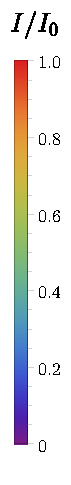
\includegraphics[scale=.77, trim={00 00 00 00}, clip]{2-Resultados/figs/0-IBar_v}};
\node[above, inner sep=0pt] (r) at (7.15,3.2) {$R$};
\end{tikzpicture}\vspace*{-.5em}
	\caption{Gráficas de la reflectancia para una FSM como función del ángulo de incidencia $\theta_i$ y tanto de la longitud de onda $\lambda$ (escala inferior), como de la energía del haz incidente en unidades de $\hbar\omega$ (escala superior), para una función dieléctrica tipo Drude con $\hbar\omega_p=4. 3$ eV  y  $\hbar\gamma=0. 15$ eV.  Las gráficas   en el renglón superior [$\mathbf{i)-v)}$]  muestran los resultados de reflectancia para  polarización \emph{p} y las del renglón inferior  [$\mathbf{i)-v)}$] para polarización  \emph{s}, donde se consideraron NPs de radio $a=30$ nm y distintas fracciones de cubierta $\Theta$: $0. 05$, $0. 1$, $0. 2$, $0. 3$ y $0. 4$. Las líneas verticales punteadas verdes y rosas corresponden a las SP-SPRs dipolar ($658$ nm) y cuadrupolar ($561$ nm), respectivamente.}	\label{fig:R-FSM}	
	\end{figure}		
					
La reflectancia para polarización \emph{p} [Fig. \ref{fig:R-FSM} $\mathbf{i)-v)}$] es cero para el ángulo de Brewster $\theta_B = 45^\circ$ y para regiones alejadas de las SP-SPRs (líneas punteadas verticales verde y rosa  localizadas en $658$ nm y $561$ nm, respectivamente). En la gráfica \textbf{v)}, $\Theta=0.4$,  se observa a $561$ nm (escala inferior) y $\theta_i>50^\circ$ que $R\approx 0$ sin embargo, la reflectancia aumenta para longitudes de onda mayores y menores a $658$ nm. Conforme la fracción de cubierta disminuye, gráficas \textbf{iii)} y \textbf{iv)}, la extinción de luz a $561$ nm  es menos evidente y para las fracciones de cubierta $\Theta=0.1$ y $0.05$, gráficas \textbf{ii)} y \textbf{i)}, ya no es apreciable la extinción de luz a la frecuencia de la SP-SPR dipolar. En contraparte, para polarización \emph{s} [Fig. \ref{fig:R-FSM} $\mathbf{vi)-x)}$] la reflectancia es apreciable para todo ángulo de incidencia a las frecuencias de las SP-SPRs. 

Para comparar la respuesta EM  de una FSM al variar la fracción de cubierta, se grafican en la  Fig. \ref{fig:FSM-Cuts} cortes de la reflectancia para $\theta_i = 65^\circ$, ángulo en donde se extingue la luz reflejada al rededor de la SP-SPR dipolar para fracciones de cubierta $\Theta>0.2$ en la Fig. \ref{fig:R-FSM}. Se muestran cortes de la reflectancia tanto para un haz incidente con polarización \emph{p} $R_p$ [Fig. \ref{sfig:FSM-cutp}], como uno con polarización \emph{s} $R_s$ [Fig. \ref{sfig:FSM-cuts}]. Para la polarización \emph{p} se presenta un mínimo en la reflectancia alrededor de $658$ nm para fracciones de cubierta mayores a $\Theta = 0.05$. Los mínimos de $R_p$ a la frecuencia de la SP-SPR dipolar son más pronunciados conforme aumenta la fracción de cubierta sin embargo, para $\Theta=0.05$ se observa un máximo en lugar de un mínimo. Para polarización \emph{s}, se presenta un máximo en la reflectancia a $658$ nm para todos los valores de $\Theta$. Para las fracciones de cubierta mayores, $\Theta = 0.3$ y $\Theta = 0.4$,  se observa un  mínimo en la reflectancia alrededor de $561$ nm para ambas polarizaciones, lo que corresponde a la SP-SPR cuadrupolar.

		\begin{figure}[h!]\centering\hspace*{-1.5em}
	\begin{subfigure}{.01\linewidth}\caption{}\label{sfig:FSM-cutp}\vspace{4.5cm}\end{subfigure}
	\begin{subfigure}{.45\linewidth}\hspace*{-1.5em}
	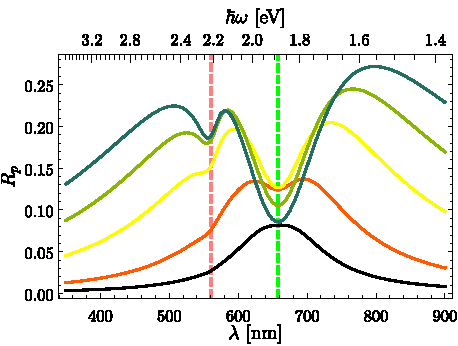
\includegraphics[scale=1]{2-Resultados/figs/4-Wp4FSMThetaVar/cut_angle_65_p.pdf}\end{subfigure}
	\begin{subfigure}{.01\linewidth}\caption{}\label{sfig:FSM-cuts}\vspace{4.5cm}\end{subfigure}\hspace*{-1.em}
	\begin{subfigure}{.45\linewidth}\centering
	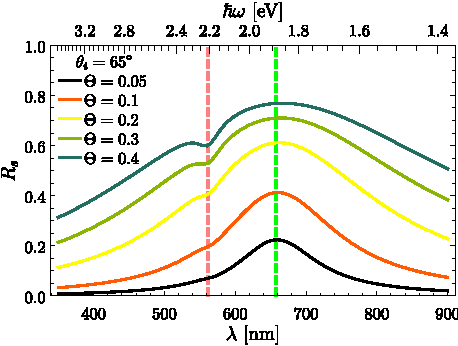
\includegraphics[scale=1 ]{2-Resultados/figs/4-Wp4FSMThetaVar/cut_angle_65_s.pdf}\end{subfigure}\vspace*{-.5em}
	\caption{Cortes de la Fig. \ref{fig:R-FSM} a $\theta_i = 65^\circ$ de reflectancia de una FSM de NPs esféricas de radio $a=30$ nm en polarización \textbf{a)} \emph{p} y \textbf{b)} \emph{s} como función tanto de la longitud de onda $\lambda$ (escala inferior), como de la energía del haz incidente en unidades de $\hbar\omega$ (escala superior). Los parámetros de la función dieléctrica tipo Drude para las NPs son $\hbar\omega_p = 4.3$ eV y $\hbar\gamma = 0.15$ eV y las fracciones de cubierta consideradas fueron $\Theta$: $0. 05$, $0. 1$, $0. 2$, $0. 3$ y $0. 4$. Las líneas verticales punteadas verdes y rosas corresponden a las SP-SPRs dipolar ($658$ nm) y cuadrupolar ($561$ nm), respectivamente.}\label{fig:FSM-Cuts}
	\end{figure}	

Al calcular la distancia mínima promedio $\langle d_{min}\rangle$ entre las NPs  de $a = 30$ nm mediante la Tab. \eqref{tab:MeanD}, se obtiene que $\langle d_{min} \rangle = 177.8$ nm para $\Theta = 0.05$. El análisis de una partícula individual es válido para el caso de $\Theta=0.05$ (en negro en la Fig. \ref{fig:FSM-Cuts}), debido a la distancia promedio entre las NPs, por tanto, la presencia del máximo en la reflectancia en la SP-SPRs dipolar (línea punteada vertical verde) corresponde a una cota mínima en $R_p$ debido al esparcimiento de cada una de las NPs; como se observa en las gráficas de las eficiencias de extinción y de esparcimiento graficadas en la Fig. \ref{fig:QextDrude}.

En las Figs. \ref{fig:R-FSM} y \ref{fig:FSM-Cuts} se observa la respuesta EM de una monocapa de NPs suspendida en un medio con $n_m=1.5$ al interactuar con una onda plana. Si se considera la presencia de un sustrato que soporte la monocapa, se puede estar en configuraci\'on de incidencia externa o interna, seg\'un sea el medio de incidencia de la onda plana. Para incidencia externa, a todo ángulo de incidencia,  una onda plana ilumina a las NPs de la monocapa por lo que, respecto al caso de la FSM, la posición de los máximos y mínimos de la reflectancia no cambiarán y los valores de $R$ presentarán un decrecimiento, debido al sustrato que disminuye el contraste entre índice de refracción de las NPs en la monocapa y el medio de transmisión. Por otro lado, para el caso de incidencia interna y ángulos mayores al ángulo crítico $\theta_c = \arcsin(n_m/n_s)$, las NPs en la monocapa son iluminadas por ondas evanescentes, por tratarse de un configuración en ATR, por lo que es posible  observar cambios en la respuesta EM de la monocapa, como sucede  cuando se tiene una placa continua y se excitan plasmones polaritones de superficie.

	\subsection{Reflectancia y transmitancia de una monocapa soportada sobre un sustrato en configuración de reflexión total atenuada}
	\label{ssection:DrudeATR}

La respuesta EM de una monocapa de NPs, suspendida en una matriz con índice de refracción $n_m$ y soportada por un sustrato con índice de refracción $n_s$, se calcula al emplear la Ec.  \eqref{eq:R} con el coeficiente de amplitud de reflexión $r$ de la Ec.  \eqref{seq:rCSMATR}. Para comparar los resultados de la reflectancia $R$ para una FSM y una monocapa en configuración ATR, se emplean los parámetros utilizado en los cálculos de las Figs. \ref{fig:R-FSM} y \ref{fig:FSM-Cuts} ($n_m=1.33$ , $a=30$ nm, $\hbar\omega_p=4.3$ eV y  $\hbar\gamma = 0.15$ eV) considerando un sustrato con índice de refracción $n_s=1.5$, pues el índice de refracción del vidrio BK7 es $n_{BK7}=1.50\pm 0.05$ en un intervalo de longitud de onda entre $334.1$ nm y $2,325.4$ nm \cite{schott2019datasheet}. En la Fig.  \ref{fig:R-ATR4} se presentan los resultados de la reflectancia $R$ en función del ángulo de incidencia $\theta_i$ y tanto de la longitud de onda $\lambda$ del haz incidente (escala inferior) como de la energía del haz $\hbar\omega$ (escala superior). Las gráficas \textbf{i) -- v}) en la Fig. \ref{fig:R-ATR4}  corresponden a la polarización \emph{p}, mientras que las gráficas \textbf{vi) -- x)} a polarización \emph{s}. Al igual que para la FSM, se consideraron los casos para la fracción de cubierta $\Theta = 0.05,\,0.1,\,0.2,\,0.3$ y $0.4$. Las SP-SPRs corresponden a la línea vertical verde punteada en $\lambda \approx 658$ nm para el modo dipolar y la línea vertical rosa punteada en  $\lambda \approx 561$ nm para el modo cuadrupolar. Adicionalmente, los puntos amarillos en la Fig. \ref{fig:R-ATR4} corresponden a los mínimos en $R$ para ángulos mayores al ángulo crítico entre el sustrato y la matriz ($\theta_c\approx 62.5^\circ$) y longitudes de onda mayores a la SP-SPR dipolar.

	\begin{figure}[h!]\centering
\begin{tikzpicture}
\node[inner sep=0pt] (graf) at (-.1,0){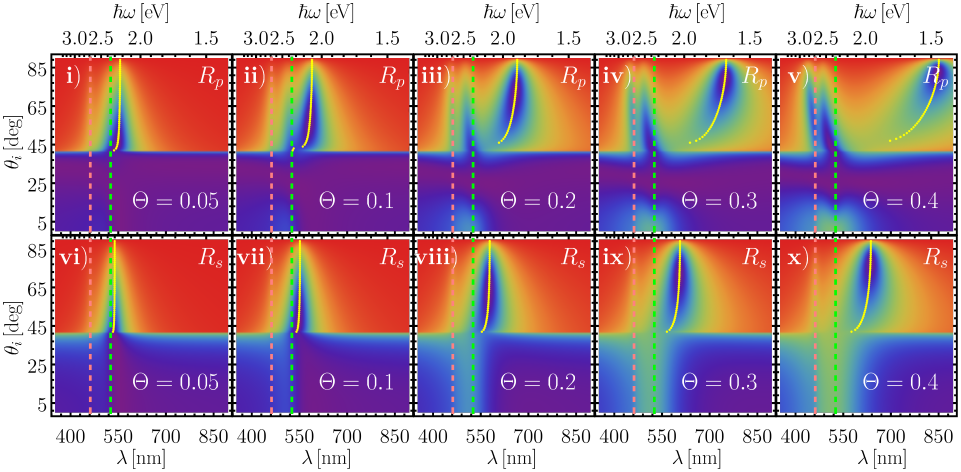
\includegraphics[width = .9\linewidth]{2-Resultados/figs/1-Wp4ThetaVar/0-2D_Grid}};
\node[right, inner sep=0pt] (legend) at (7,.05) {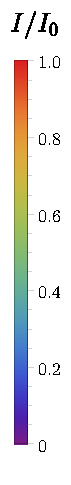
\includegraphics[scale=.77, trim={00 00 00 00}, clip]{2-Resultados/figs/0-IBar_v}};
\node[above, inner sep=0pt] (r) at (7.15,3.2) {$R$};
\end{tikzpicture}\vspace*{-.5em}
	\caption{Gráficas de la reflectancia de una monocapa en configuración ATR como función del ángulo de incidencia $\theta_i$ y de la longitud de onda $\lambda$ (escala inferior) así como de la energía del haz incidente en unidades de $\hbar\omega$ (escala superior), para una función dieléctrica tipo Drude con $\hbar\omega_p=4. 3$ eV  y  $\hbar\gamma=0. 15$ eV.  Las gráficas   en el renglón superior [$\mathbf{i)-v)}$]  muestran los resultados de reflectancia para  polarización \emph{p} y las del renglón inferior  [$\mathbf{vi)-x)}$] para polarización  \emph{s}, donde se consideraron NPs de radio $a=30$ nm y distintas fracciones de cubierta $\Theta$: $0. 05$, $0. 1$, $0. 2$, $0. 3$ y $0. 4$. Las líneas verticales punteadas verdes y rosas corresponden a las SP-SPRs dipolar ($658$ nm) y cuadrupolar ($561$ nm), respectivamente.	os puntos amarillos corresponden a los mínimos en $R$ para ángulos mayores a $\theta_c\approx 62.5^\circ$ y longitudes de onda mayores a la SP-SPRs dipolar.}	\label{fig:R-ATR4}	
	\end{figure}	

En la Fig.  \ref{fig:R-ATR4} se observa que $R\approx 1$ para ángulos mayores al ángulo crítico, $\theta_c \approx 62.5^\circ $ excepto en dos regiones: a las longitudes de onda correspondientes a las SP-SPRs (líneas punteadas verticales) y en una región a longitudes de onda mayores a la SP-SPR dipolar (puntos amarillos). La disminución en la reflectancia después del ángulo crítico alrededor de la SP-SPR cuadrupolar ($561$ nm) es resultado de la extinción de luz debido a la presencia de las NPs y es apreciable tanto para polarización \emph{p} como para \emph{s}, siendo más evidente para las fracciones de cubierta consideradas mayores. Por ejemplo, en el panel superior de la Fig. \ref{fig:R-ATR4},  la excitación cuadrupolar de una sola partícula es apreciable en $\lambda \approx 658$ nm cuando $R_p$ disminuye para $\Theta = 0.4$, gráfica  $\mathbf{v)}$, en comparación a $\Theta = 0.05$, $\mathbf{i)}$. A pesar de que este comportamiento es análogo para la polarización \emph{s}, panel inferior de la  Fig. \ref{fig:R-ATR4}, los valores de $R_s$ a las frecuencias de las SP-SPRs son mayores que los de $R_p$, como se observa al comparar las gráficas de los cálculos con $\Theta=0.3$: \textbf{iv)} para $R_p$ y \textbf{ix)} para $R_s$.

La respuesta óptica de la monocapa a $658$ nm es distinto para cada polarización. Mientras que en polarización \emph{p}, gráficas \textbf{i)}-\textbf{v)}, la SP-SPR dipolar se aprecia para todos los valores de $\Theta$ escogidos, para polarización \emph{s}, gráficas \textbf{vi)}-\textbf{x)}, esto sólo ocurre cuando $\Theta$ toma valores cercanos a cero. Adicional a la región cercana a las SP-SPRs, se observan mínimos en la reflectancia para ángulos de incidencia mayores al ángulo crítico y para longitudes de onda mayores a la SP-SPR dipolar, los cuales están  representados por los puntos amarillos en la Fig. \ref{fig:R-ATR4}. Dado que los puntos amarillos corresponden a una excitación que ocurre energías  menores en comparación a las SP-SPRs, ésta no puede ser plasmónica de partícula individual,  por lo que especula que se debe a una respuesta colectiva como la resonancia de red del plasmón de superficie (Plasmon Surface Lattice Resonance, PSLR) reportada en \cite{danilov2018ultra}. Al comparar las gráficas en la  Fig.  \ref{fig:R-ATR4} se observa que la posible excitación colectiva se corre al rojo  conforme aumenta la fracción de cubierta $\Theta$, o bien, que para valores de $\Theta$ cercanos a cero se comporta como la SP-SPR dipolar, comportamiento más evidente en polarización \emph{p} que en \emph{s} [ver \textbf{ii)} y \textbf{vi)} y \textbf{x)}]


\begin{figure}[h!]\centering\hspace*{-1.5em}
	\begin{subfigure}{.01\linewidth}\caption{}\label{sfig:R-ATR4-cutp}\vspace{4.5cm}\end{subfigure}
	\begin{subfigure}{.45\linewidth}\hspace*{-1.5em}
	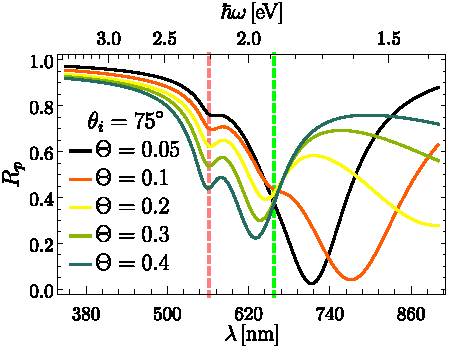
\includegraphics[scale=1]{2-Resultados/figs/1-Wp4ThetaVar/cut_angle_75_p.pdf}\end{subfigure}
	\begin{subfigure}{.01\linewidth}\caption{}\label{sfig:R-ATR4-cuts}\vspace{4.5cm}\end{subfigure}\hspace*{-1.em}
	\begin{subfigure}{.45\linewidth}\centering
	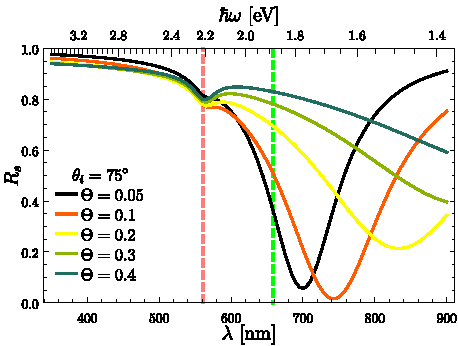
\includegraphics[scale=1 ]{2-Resultados/figs/1-Wp4ThetaVar/cut_angle_75_s.pdf}\end{subfigure}\vspace*{-.5em}
	\caption{Cortes de la Fig. \ref{fig:R-ATR4} a $\theta_i = 75^\circ$ de reflectancia de una monocapa en configuración ATR de NPs esféricas de radio $a=30$ nm en polarización \textbf{a)} \emph{p} y \textbf{b)} \emph{s} como función de la longitud de onda $\lambda$ (escala inferior) y de la energía $\hbar\omega$ (escala superior). Los parámetros de la función dieléctrica tipo Drude para las NPs son $\hbar\omega_p = 4.3$ eV y $\hbar\gamma = 0.15$ eV y las fracciones de cubierta consideradas fueron $\Theta$: $0. 05$, $0. 1$, $0. 2$, $0. 3$ y $0. 4$. Las líneas verticales punteadas verdes y rosas corresponden a las SP-SPRs dipolar ($658$ nm) y cuadrupolar ($561$ nm), respectivamente. }\label{fig:R-ATR4-Cuts}
	\end{figure}	  

Dado que la presunta excitación colectiva presenta un mínimo en la reflectancia  al rededor de $\theta_i = 75^\circ$ para los casos de fracción de cubierta analizados en la Fig.  \ref{fig:R-ATR4}, se presentan cortes de la reflectancia a este ángulo en la Fig. \ref{fig:R-ATR4-Cuts}, en donde las líneas punteadas verticales corresponden a las longitudes de onda de las SP-SPRs (verde para la excitación dipolar y rosa para la cuadrupolar). En polarización \emph{p}, Fig. \ref{sfig:R-ATR4-cutp}, y polarización \emph{s}, la excitación de la monocapa para todos los valores de $\Theta$ alrededor de $\lambda \approx 561$ nm coincide con la SP-SPR cuadrupolar.  La reflectancia a la longitud de onda de la SP-SPR cuadrupolar disminuye conforme la fracción de cubierta crece, por lo que se relaciona con la cantidad de NPs presentes en la monocapa. De forma distinta, la excitación dipolar de partícula individual ($658$ nm) no se aprecia para todos los casos estudiados en la Fig. \ref{fig:R-ATR4-Cuts} y sólo coincide para $\Theta=0.3$ nm; para $0.2\leq \Theta$ se presenta un corrimiento al azul de la SP-SPR dipolar, mientras que para $\Theta=0.05$ (línea sólida negra) se corre al rojo, empalmándola con el presunto modo colectivo de la monocapa. El mínimo en la reflectancia a $\lambda\approx 715$ nm  se atribuye al modo colectivo y no a la SP-SPR debido a que el la reflectancia toma valores cercanos a cero, comportamiento no spreciable para los corrimientos al azul de la SP-SPR dipolar. Para el caso de polarización \emph{s}, no hay corrimientos al azul de la SP-SPR dipolar, sino sólo se aprecia el presunto modo colectivo a $\lambda>658$ nm.

Los mínimos a $\lambda>650$ nm, que corresponden al presunto modo colectivo, presentan un corrimiento al rojo conforme la fracción de cubierta de la monocapa aumenta  para ambas polarizaciones, contrario al comportamiento observado en las excitaciones dipolares de partícula individual de la monocapa observadas en la Fig. \ref{sfig:R-ATR4-cutp} entre $561$ nm y $658$ nm. Otra diferencia entre las excitaciones en $\lambda$ mayores a las SP-SPRs y los corrimientos al azul de éstas, es que la disminución en el valor de $R$ no es monótona, sino que el decrecimiento en $R$ es máximo a fracciones de cubierta medias. Por lo anterior, los mínimos en $R_p$ y $R_s$ localizados a longitudes de onda mayores a la de los modos plasmónicos de partícula individual no son corrimientos de las excitaciones multipolares de una partícula, sino una probable respuesta colectiva de las NPs en la monocapa. El corrimiento al rojo del modo colectivo es mayor para  polarización \emph{p} que para \emph{s}, como se observa para $\Theta=0.1$ (línea naranja sólida), en donde al mínimo en $R$ se localiza a $765$ nm para \emph{p} y  a $740$ nm para \emph{s}.

\begin{figure}[t!]\centering
\begin{tikzpicture}
\node[inner sep=0pt] (graf) at (-.1,0){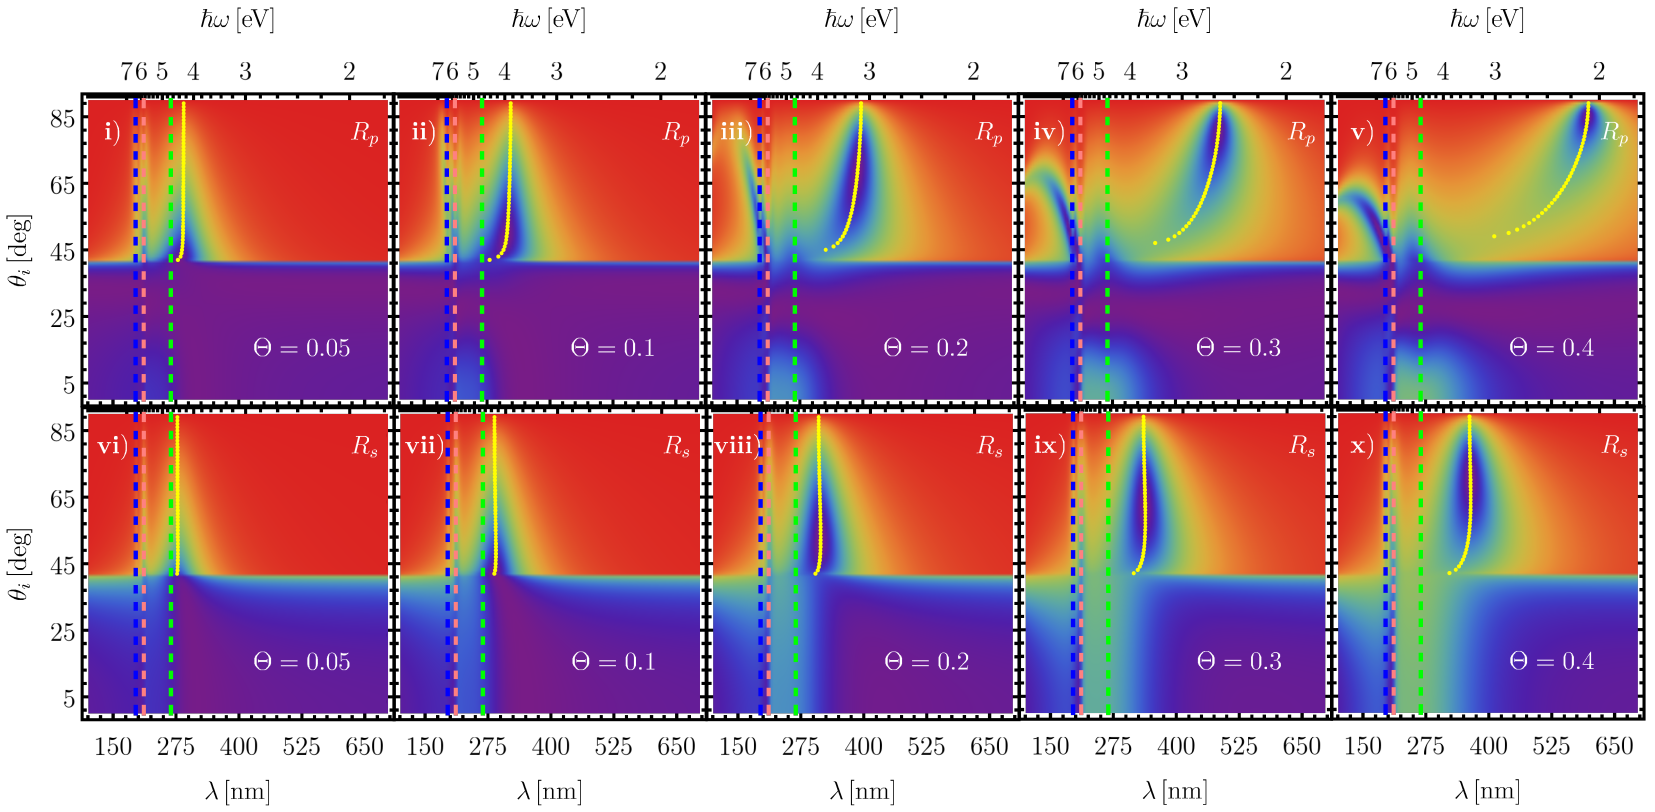
\includegraphics[width = .9\linewidth]{2-Resultados/figs/2-Wp10ThetaVar/0-2D_Grid}};
\node[right, inner sep=0pt] (legend) at (7,.05) {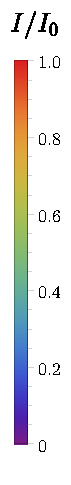
\includegraphics[scale=.77, trim={00 00 00 00}, clip]{2-Resultados/figs/0-IBar_v}};
\node[above, inner sep=0pt] (r) at (7.15,3.2) {$R$};
\end{tikzpicture}\vspace*{-.5em}
	\caption{Gráficas de la reflectancia de una monocapa en configuración ATR como función del ángulo de incidencia $\theta_i$ y de la longitud de onda $\lambda$ (escala inferior), así como de la energía del haz incidente en unidades de $\hbar\omega$ (escala superior), para una función dieléctrica tipo Drude con $\hbar\omega_p=10$ eV  y  $\hbar\gamma=0. 15$ eV.  Las gráficas   en el renglón superior [$\mathbf{i)-v)}$] muestran los resultados  para  polarización \emph{p} y las del renglón inferior  [$\mathbf{vi)-x)}$] para polarización  \emph{s}, donde se consideraron NPs de radio $a=30$ nm y distintas fracciones de cubierta $\Theta$: $0. 05$, $0. 1$, $0. 2$, $0. 3$ y $0. 4$. Las líneas verticales punteadas verdes, rosas y cianes corresponden a las SP-SPRs dipolar ($342$ nm), cuadrupolar ($262$ nm) y octopolar ($195$ nm), respectivamente.  Los puntos amarillos corresponden a los mínimos en $R$ para ángulos mayores a $\theta_c\approx 62.5^\circ$ y longitudes de onda mayores a la SP-SPRs dipolar. }	\label{fig:R-ATR10}	
	\end{figure}	
	
Para $\Theta = 0.3$ y $0.4$, el presunto modo colectivo se separa de la SP-SPRs dipolar (línea punteada vertical verde) a longitudes mayores a $900$ nm, por lo que 
no son apreciables en la Fig. \ref{fig:R-ATR4-Cuts}. Sin embargo, al escoger valores de $\Theta$ entre $0.05$ y $0.2$, es posible sintonizar la resonancia del presunto modo colectivo entre $715$ nm y $890$ nm para polarización \emph{p}, o bien, entre $715$ y $815$ para polarización \emph{s}. Si el presunto modo colectivo depende no sólo de la fracción de cubierta de la monocapa, sino también del material de las NPs, su posición cambiará al incrementar la frecuencia de plasma en el modelo de Drude, que caracteriza la respuesta EM de las NPs y modifica la posición de las SP-SPRs: al considerar $\hbar\omega_p = 10$ eV las SP-SPRs se corren al azul. Los resultados de la reflectancia de un sistema monocapa con los parámetros empleados en la Fig. \ref{fig:R-ATR4}, pero con $\hbar\omega_p = 10$ eV, se muestran en la Fig. \ref{fig:R-ATR10}. Las líneas verticales punteadas verde y rosa en $342$ nm y $262$ nm corresponden a las SP-SPRs dipolar y cuadrupolar,respectivamente, mientras que los puntos amarillos corresponden al presunto modo colectivo .
				
	
En las gráficas mostradas en la Fig. \ref{fig:R-ATR10} ($\hbar\omega_p = 10$ eV) se aprecian características semejantes a las observadas en la Fig. \ref{fig:R-ATR4} donde se empleó $\hbar\omega_p = 4.3$ eV. La excitación de la SP-SPR dipolar (líneas verticales punteadas rosas) sólo es apreciable para polarización \emph{p} y para $\Theta = 0.05$ para polarización  \emph{s}. Para ambas polarizaciones la reflectancia disminuye para $\theta_i>\theta_c=62.5^\circ$ y valores de $\lambda$ cercanos a la SP-SPR cuadrupolar (líneas verticales punteadas rosas), así como en longitudes de onda mayoes a la SP-SPR dipolar, es decir, en la presunta excitación colectiva  (puntos amarillos); de igual forma, el corrimeinto al rojo de la presunta excitación colectiva respecto a la SP-SPR dipolar es mayor para polarización \emph{p} que para \emph{s}.  Asimismo, al modificar el parámetro $\hbar\omega_p$ de $4.3$ eV a $10$ eV se sintonizó la presunta excitación colectiva a longitudes de onda menores, por ejemplo, para $\Theta = 0.3$, para todo ángulo de incidencia $\theta_i$, la presunta excitación colectiva se encuentra a $\lambda<900$ nm para $\hbar\omega_p=10$ eV, mientras que para $\hbar\gamma=4.3$ eV el modo colectivo ya no se apreciaba en el espectro visible, como se puede observar en las gráficas \textbf{iv)} y \textbf{ix)} de las Figs. \ref{fig:R-ATR4} y \ref{fig:R-ATR10}.

Dado que la elección del parámetro $\omega_p$ sintoniza tanto las SP-SPRs como el presunto modo colectivo, la separación entre estos puede modificarse. Para comparar con el caso de $\hbar\omega_p=4.3$ eV [Fig. \ref{fig:R-ATR4-Cuts}], se grafica en la Fig. \ref{fig:R-ATR10-Cuts} cortes de la reflectancia graficada en la Fig. \ref{fig:R-ATR10}, donde se emplea $\hbar\omega_p = 10$ eV, a $\theta_i = 75^\circ$ para ambas polarizaciones,  Fig. \ref{sfig:R-ATR10-cutp} para \emph{p} y Fig. \ref{sfig:R-ATR10-cuts} para \emph{s}, en  función de la longitud de onda, para una monocapa de NPs de radio $a= 30$ nm  y fracciones de cubierta consideradas en la Fig. \ref{fig:R-ATR10}; las líneas punteadas verde y rosa  corresponden a las SP-SPRs dipolar y cuadrupolar, respectivamente. Para ambas polarizaciones y para todas las fracciones de cubierta, se presenta una excitación a la longitud de onda correspondiente a la SP-SPR octopolar $\lambda=240$ nm, la cual se corre al azul para polarización \emph{p} pero no para \emph{s}, al igual que  la SP-SPR cuadrupolar al rededor de $262$ nm (línea punteada vertical rosa). De forma semejante a la elección del parámetro $\hbar\omega_p = 4.3$ eV, para $\hbar\omega_p=10$ eV la reflectancia de la monocapa a $\theta_i=75^\circ$ (Fig. \ref{fig:R-ATR4-Cuts}) para $0.2\leq\Theta$, se presenta un corrimiento al azil de la SP-SPR dipolar (línea punteada vertical verde). Para $\Theta=0.05$ y $0.1$, también para polarización \emph{p}, al igual que para todos los valores de $\Theta$ para \emph{s}, no se distingue la SP-SPR dipolar, sino que se presenta el presunto modo colectivo a longitudes de onda mayores a $342$ nm.

\begin{figure}[h!]\centering\hspace*{-1.5em}
	\begin{subfigure}{.01\linewidth}\caption{}\label{sfig:R-ATR10-cutp}\vspace{4.5cm}\end{subfigure}
	\begin{subfigure}{.45\linewidth}\hspace*{-1.5em}
	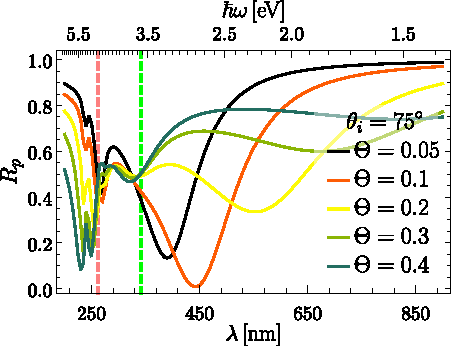
\includegraphics[scale=1]{2-Resultados/figs/2-Wp10ThetaVar/cut_angle_75_p.pdf}\end{subfigure}
	\begin{subfigure}{.01\linewidth}\caption{}\label{sfig:R-ATR10-cuts}\vspace{4.5cm}\end{subfigure}\hspace*{-1.em}
	\begin{subfigure}{.45\linewidth}\centering
	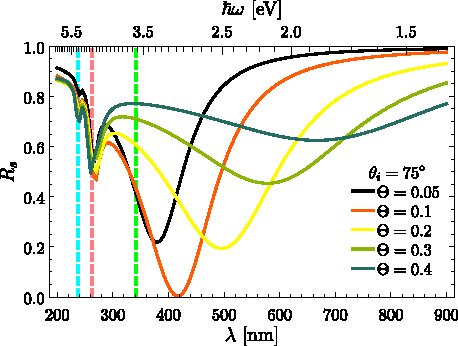
\includegraphics[scale=1 ]{2-Resultados/figs/2-Wp10ThetaVar/cut_angle_75_s.pdf}\end{subfigure}\vspace*{-.5em}
	\caption{Cortes de la Fig. \ref{fig:R-ATR10} a $\theta_i = 75^\circ$ de reflectancia de una monocapa en configuración ATR de NPs esféricas de radio $a$ en polarización \textbf{a)} \emph{p} y \textbf{b)} \emph{s} como función de la longitud de onda $\lambda$ (escala inferior) y de la energía en unidades de $\hbar\omega$ (escala superior). Los parámetros de la función dieléctrica tipo Drude para las NPs son $\hbar\omega_p = 10$ eV y $\hbar\gamma = 0.15$ eV y las fracciones de cubierta consideradas fueron $\Theta$: $0. 05$, $0. 1$, $0. 2$, $0. 3$ y $0. 4$. Las líneas verticales punteadas verdes, rosas y cianes corresponden a las SP-SPRs dipolar ($342$ nm), cuadrupolar ($262$ nm) y octopolar ($195$ nm), respectivamente.  }\label{fig:R-ATR10-Cuts}
	\end{figure}	

Los mínimos en la reflectancia en $\lambda > 342$ nm se atribuyen a una respuesta colectiva. Las excitaciones del presunto modo colectivo con $\hbar\omega_p = 10$ eV se comportan de manera análoga al caso de $\hbar\omega_p = 4.3$ eV: se corren al rojo conforme aumenta la fracción de cubierta y su presencia es más evidente para fracciones de cubierta media, siendo  $\Theta=0.2$ cuando la reflectancia en la excitación del presunto modo colectivo alcanza el valor mínimo de reflectancia. Cuando $\Theta = 0.05$ (líneas negras en la Fig. \ref{fig:R-ATR10-Cuts}) la excitación del presunto modo colectivo se separa de la SP-SPR dipolar   $40$ nm para ambas polarizaciones mientras que para $\Theta = 0.2$ la excitación del presunto modo colectivo se separa de la SP-SPR dipolar  $120$ nm y $100$ nm para polarización \emph{p} y \emph{s}, respectivamente, es decir, que la separación entre ambas excitaciones es menor que cuando se consideró $\hbar\omega_p = 4.3$ eV en la Fig. \ref{fig:R-ATR4-Cuts} (en donde para $\Theta=0.2$ la presunta excitación colectiva se separó de la SP-SPR dipolar más de $240$ nm). Sin embargo, la anchura a media altura (Full Width at Half Maximum, FWHM) $\Delta\lambda_{FWHM}$ de la presunta excitación colectiva es mayor para $\hbar\omega_p=10$ eV en comparación a $\hbar\omega_p=4.3$ eV. Por ejemplo, para $\Theta = 0.05$ y $\hbar\omega_p = 4.3$ eV,  $\Delta\lambda_{FWHM}\approx 200$ nm para polarización \emph{p} y  $\Delta\lambda_{FWHM}\approx 100$ nm para  \emph{s} (ver Fig. \ref{fig:R-ATR4-Cuts}), mientras que para  $\hbar\omega_p = 10$ eV,  $\Delta\lambda_{FWHM}\approx 300$ nm para polarización \emph{p} y  $\Delta\lambda_{FWHM}\approx 130$ nm para  \emph{s} (ver Fig. \ref{fig:R-ATR10-Cuts}).

%Para polarización \emph{p}, adicional a las SP-SPRs de orden $\ell = 2,\,3$ y $4$ se observa una excitación que se localiza en la longitud de onda de la SP-SPR octopolar para $\Theta=0.05$ y se corre al azul conforme aumenta la fracción de cubierta, hasta localizarse en $\lambda= 135$ nm para $\Theta=0.4$ [ver línea vertical punteada azul en laFig. \ref{sfig:R-ATR10-cutp}]. La excitación a $\lambda<185$ en polarización \emph{p} tomo un valor mínimo en la reflectancia cuando $\Theta=0.2$, una fracción de cubierta media. Esta excitación corresponde a la ramificación también presente en las gráficas \textbf{iii)} a \textbf{v)} de la Fig. \ref{fig:R-ATR10}. Ya que se observó una segunda respuesta que no corresponde a las SP-SPRs, sino que sigue las tendencias del presunto modo colectivo, se especula que es un complemento  de ellas, dado que las  PSLRs reportadas en \cite{danilov2018ultra} son, para un sistema determinado, dos excitaciones que se corren al rojo y al azul. Es decir, que tanto el modo que se corre al azul a $\lambda<185$ nm [línea punteada azul en la Fig. \ref{sfig:R-ATR10-cutp}], como el presunto modo colectivo (puntos amarilos en la Fig. \ref{fig:R-ATR10}) se pueden relacionar con las PSLRs.  

 Ya que el presunto modo colectivo sufre un corrimiento al rojo al aumentar la fracción de cubierta, se analizó si el comportamiento es semejante a cambios en el radio $a$ de las NPs.  Este análisis se llevó a cabo dado que tanto el radio $a$ como la fracción de cubierta $\Theta$ modifican el volumen neto de material plasmónico, es decir, la cantidad de electrones libres en la monocapa aumenta, así como la distancia mínima promedio $\langle d_{min}  \rangle$ entre las NPs. Si  los mínimos en $R$  a energías menores que la de la SP-SPR dipolar son sensibles al radio de las NPs, como lo son con la fracción de cubierta, se corrobora que esta excitación se debe a un efecto colectivo de las NPs.
 
Los resultados de la reflectancia de una monocapa con $\Theta=0.3$, inmersa en un medio con índice de refracción $n_m = 1.5$ y soportada por un sustrato con índice de refracción $n_m= 1.5$, se muestran en la Fig.  \ref{fig:R-RVar}, como función del ángulo de incidencia, tanto de la longitud de onda $\lambda$ (escala inferior) como de la  energía $\hbar\omega$ (escala superior) del haz incidente. Se consideraron NPs  con una respuesta EM dada dada por una función dieléctrica  tipo Drude [Ec. \eqref{eq:Drude}] con los parámetros $\hbar\omega_p =4.3$ eV y $\hbar\gamma=0.15$ eV, cuyos radios $a$ fueran los siguientes: $3$ nm, $5$ nm, $10$ nm y $20$ nm. La reflectancia en polarización \emph{p} se presenta en las gráficas $\mathbf{i)-iv)}$,mientras que en \emph{s}, en las gráficas $\mathbf{v)-viii)}$. Las SP-SPRs dipolar y cuadrupolar corresponden a las líneas punteadas verde y rosa, respectivamente. Para $a = 3$ nm y $5$ nm la excitación dipolar se localiza en $\lambda\approx 615$ nm, para el radio  $a = 10$ nm en $\lambda\approx 620$ nm y $a=20$ nm en $\lambda\approx 635$ nm, mientras que la SP-SPR cuadrupolar se localiza en $551$ nm para $a\leq 10$ nm y para el caso  $a=20$ nm, $\lambda = 555$ nm.

	\begin{figure}[h!]\centering
\begin{tikzpicture}
\node[inner sep=0pt] (graf) at (0,0){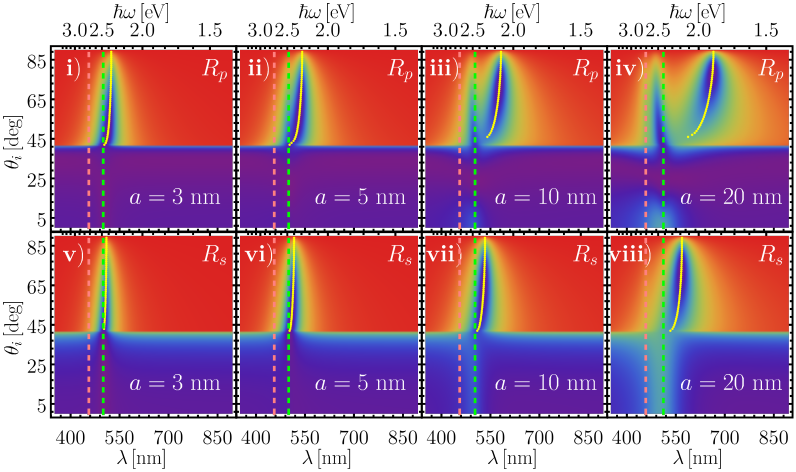
\includegraphics[width = .76\linewidth]{2-Resultados/figs/3-Wp4rVar/0-2D_Grid}};
\node[right, inner sep=0pt] (legend) at (6,.05) {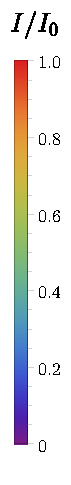
\includegraphics[scale=.8, trim={00 00 00 00}, clip]{2-Resultados/figs/0-IBar_v}};
\node[above, inner sep=0pt] (r) at (6.2,3.2) {$R$};
\end{tikzpicture}\vspace*{-.5em}
	\caption{Gráficas de la reflectancia de una monocapa en configuración ATR como función del ángulo de incidencia $\theta_i$ y de la longitud de onda $\lambda$ (escala inferior), así como de la energía del haz incidente en unidades de $\hbar\omega$ (escala superior), para una función dieléctrica tipo Drude con $\hbar\omega_p=4.3$ eV  y  $\hbar\gamma=0. 15$ eV.  Las gráficas   en el renglón superior [$\mathbf{i)-v)}$] muestran los resultados para  polarización \emph{p} y las del renglón inferior  [$\mathbf{vi)-x)}$]  para polarización  \emph{s}, donde se consideró una fracción de cubierta $\Theta = 0.3$ y  NPs de radio  $a$: $3$ nm, $5$ nm, $10$ nm y $20$ nm.  Las líneas verticales punteadas verdes y rosas corresponden a las SP-SPRs dipolar y  cuadrupolar, respectivamente.  Los puntos amarillos corresponden a los mínimos en $R$ para ángulos mayores a $\theta_c\approx 62.5^\circ$ y longitudes de onda mayores a la SP-SPRs dipolar.
}	\label{fig:R-RVar}	
	\end{figure}	

En la Fig.   \ref{fig:R-RVar} (variación de $a$) la respuesta EM de la monocapa es análoga al de la Fig. \ref{fig:R-ATR4} (variación de $\Theta$) puesto que se presentan  dos regiones en $\theta_i>\theta_c=62.5^\circ$  donde se cumple que $R<1$: en $\lambda$ cercanas a las SP-SPRs y en longitudes de onda mayores a la excitación dipolar de una partícula. La distancia entre estas regiones aumenta al crecer el radio de las NPs, al igual que lo hacía al aumentar la fracción de cubierta, ademas de que esta distancia es mayor para polarización \emph{p}, que para \emph{s}. Asimismo, la SP-SPR dipolar sólo es apreciable para polarización \emph{p} a partir de NPs con radios mayores a $10$ nm; para \emph{s} la resonancia sólo es apreciable para ángulos menores al ángulo crítico ($\theta_c\approx 62.5^\circ$). Dado que la excitación a energías menores a las de las SP-SPRs (puntos amarillos) se modifica al aumentar el radio de las NPs, y no solo al cambiar el valor de la fracción de cubierta, esta excitación corresponde a un modo coletivo ya que responde a la cantidad neta de material plasmónico ---es decir, de electrones libres--- presentes en la monocapa. Para analizar la respuesta EM de la monocapa al aumentar el radio de las NPs, y compararla con la variación en $\Theta$ en la Fig. \ref{fig:R-ATR4},  se grafica la reflectancia a $\theta_i = 75^\circ$. 

En la Fig. \ref{fig:R-RVar-Cuts} se presentan cortes de la reflectancia graficada en la Fig. \ref{fig:R-RVar} a $\theta_i = 75^\circ$. Dado que la longitud de onda de las SP-SPRs depende del radio de las NPs, la excitación dipolar para los tamaños de partículas utilizadas corresponde a la región verde entre $615$ nm y $635$ nm, mientras que la cuadrupolar corresponde a la región rosa entre $551$ nm y $555$ nm.
 En los resultados de la reflectancia para polarización \emph{p}, graficados en la Fig. \ref{sfig:R-RVar-cutp}, la excitación cuadrupolar sólo es apreciable para $a=20$ nm, y la SP-SPR dipolar se identifica para los radios de $10$ nm y $20$ nm (líneas amarillas y verdes) como un mínimo en $R_p$ a $\lambda\approx 620$ nm. Para $a=5$ nm, la reflectancia $\lambda\approx 620$ nm no es mínima, sin embargo se presenta un cambio en la pendiente de la reflectancia a dicha longitud de onda; adicionalmente, en $690$ nm, la reflectancia para $a=5$ nm tiene un mínimo con $R_p<0.1$, el cual se atribuye al modo colectivo. Para $a=3$ nm (línea negra) no se manifiesta la SP-SPR dipolar sino únicamente el mínimo correspondiente al modo colectivo a $650$ nm. A partir del comportamiento de $R_p$ para $a=3$ nm y $a=5$ nm a $620$ nm, así como el corrimiento al azul de la excitación del modo colectivo al aumentar el radio de las NPs en la monoca, se concluye que para NPs con radios tendiendo a cero, la excitación colectiva corresponde a la de partícula individual.
 
 Para polarización \emph{s}, Fig. \ref{sfig:R-RVar-cuts}, la respuesta cuadrupolar sólo se observa para $a = 20$ nm y, como ocurrió en casos pasados, la SP-SPR dipolar no es apreciable. Los mínimos de la reflectancia dentro del rango de la SP-SPR dipolar se corren al rojo conforme crece el radio y la disminución en el valor de $R$ es mucho menor que la disminución  observada en la Fig. \ref{sfig:R-ATR4-cutp} (respuesta EM de la monocapa de NPs tipo Drude con $\hbar\omega_p = 4.3$, $a = 30$ nm y variaciones en $\Theta$) para la SP-SPR dipolar. Las excitaciones a $\lambda>620$ nm en la Fig. \ref{fig:R-RVar-Cuts} siguen las tendencias observadas en el modo colectivo, se atribuyen a éste y se corrobora que la excitación colectiva se traslapa con la SP-SPR dipolar cuando el radio de las NPs tiende a cero, también para polarización \emph{s}.
 
\begin{figure}[h!]\centering\hspace*{-1.5em}
	\begin{subfigure}{.01\linewidth}\caption{}\label{sfig:R-RVar-cutp}\vspace{4.5cm}\end{subfigure}
	\begin{subfigure}{.45\linewidth}\hspace*{-1.5em}
	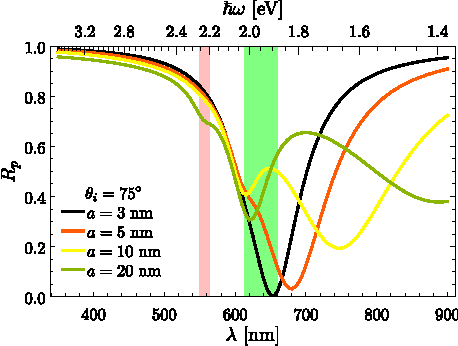
\includegraphics[scale=1]{2-Resultados/figs/3-Wp4rVar/cut_angle_75_p.pdf}\end{subfigure}
	\begin{subfigure}{.01\linewidth}\caption{}\label{sfig:R-RVar-cuts}\vspace{4.5cm}\end{subfigure}\hspace*{-1.em}
	\begin{subfigure}{.45\linewidth}\centering
	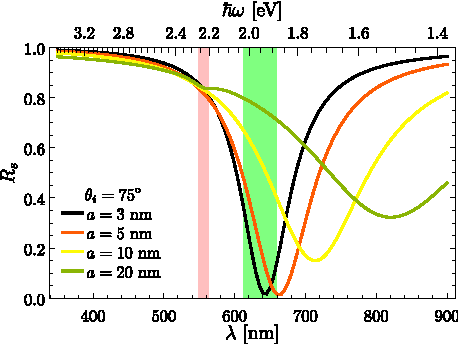
\includegraphics[scale=1 ]{2-Resultados/figs/3-Wp4rVar/cut_angle_75_s.pdf}\end{subfigure}\vspace*{-.5em}
	\caption{Cortes de la Fig. \ref{fig:R-RVar} a $\theta_i = 75^\circ$ de las gráficas de reflectancia de una monocapa en configuración ATR (Fig. \ref{fig:R-RVar}) de NPs esféricas de fracción de cubierta $\Theta = 0.3$ en polarización \textbf{a)} \emph{p} y \textbf{b)} \emph{s} en función de la longitud de onda $\lambda$ (escala inferior) y de la energía $\hbar\omega$ (escala superior). Los parámetros de la función dieléctrica tipo Drude para las NPs son $\hbar\omega_p = 4.3$ eV y $\hbar\gamma = 0.15$ eV y las fracciones de cubierta consideradas fueron $a$: $3$ nm, $5$ nm, $10$ nm y $20$ nm. La SP-SPR dipolar para los tamaños de partículas utilizadas corresponde la región verde entre $500$ nm y $512$ nm, mientras que la cuadrupolar corresponde a la región rosa entre $456$ nm y $561$ nm.}\label{fig:R-RVar-Cuts}
	\end{figure}	

La respuesta óptica de la monocapa correspondiente al modo colectivo presenta, a un valor de $\theta_i$ fijo (Figs. \ref{fig:R-ATR4-Cuts}, \ref{fig:R-ATR10-Cuts} y \ref{fig:R-RVar-Cuts}), un ensanchamiento de la excitación, así como un corrimiento al rojo de ésta, al aumentar la fracción de cubierta de la monocapa o el radio de las NPs que la conforman. La excitación colectiva también se corre al rojo al aumentar el ángulo de incidencia, como se observa en las Figs. \ref{fig:R-ATR4}, \ref{fig:R-ATR10} y \ref{fig:R-RVar} y los  valores de la reflectancia, a las longitudes de onda de la excitación colectiva, es menor conforme aumenta el ángulo de incidencia, como se evidencia en los casos con $\Theta=0.3$ y $0.4$; otro efecto en la elección del ángulo de incidencia es la disminución del ancho de la resonancia al aunmentar $\theta_i$. La SP-SPR dipolar coincide con la excitación colectiva cuando los radios de la NPs de la monocapa, o su fracción de cubierta, tienden a cero y cuando los ángulo de incidencia son cercanos al ángulo crítico $\theta_c$. Asimismo, para polarización \emph{p} la SP-SPR dipolar es apreciable en la reflectancia y distinguible del modo colectivo, mientras que para \emph{s} no se aprecia la SP-SPR dipolar.  El valor de la reflectancia a las longitudes de onda de la excitación colectiva, así como su ancho, son dependientes del material de las NPs, por ejemplo, para  $a=30$ nm y a $\theta_i=75^\circ$ $\hbar\omega_p=4.3$ eV (Fig. \ref{fig:R-ATR4-Cuts}) la reflectancia toma el valor más cercano a cero en $715$ nm al escoger  $\Theta=0.05$ pero para $\hbar\omega_p=10$ eV (Fig. \ref{fig:R-ATR10-Cuts}) esto ocurre con $\Theta=0.1$ a $\lambda=440$ nm. 

 Dado que el modo colectivo estudiado se presenta a energías menores a la de las SP-SPRs, ésta no es una excitación plasmónica, de forma semejante que las PSLRs reportadas en  \cite{kabashin2009plasmonic} y \cite{danilov2018ultra}. Sin embargo, las PSLRs son una excitación colectiva que se presenta en un arreglo ordenado de nanocilindros \cite{kabashin2009plasmonic} y \cite{danilov2018ultra} que, además, cuenta con las características de un modo guiado, es decir, que la energía se propaga a través de la monocapa de nanocilindros \cite{kabashin2009plasmonic}. El modo colectivo  para sistemas desordenados de NPs esféricas idénticas (puntos amarillos en las Figs. \ref{fig:R-ATR4}, \ref{fig:R-ATR10} y \ref{fig:R-RVar}) se caracterizó mediante los mínimos en la reflectancia a las  longitudes de onda de excitación $\lambda_{exc}$, mayores a las de las SP-SPRs. Si la transmitancia $T$ de la monocapa evaluada en $\lambda_{exc}$ no es máxima, entonces el modo colectivo presenta características de un modo guiado, semejante a las PSLRs.

 En la Fig. \ref{fig:RT-Omegas} se muestran los cálculos de la reflectancia $R$, la transmitancia $T$ y la suma de éstas ($R+T$) de una monocapa de NPs inmersa en un medio con índice de refracción $n_m=1.5$ y soportada por un sustrato con índice de refracción $n_s=1.5$, en función del ángulo de incidencia $\theta_i$, así como de la longitud de onda $\lambda$ (escala inferior) y de la energía  $\hbar\omega$ (escala superior), tanto para polarización \emph{p}  [\textbf{i)}--\textbf{iii)}] como para \emph{s} [\textbf{iv)}--\textbf{vi)}]. Fueron seleccionados para $\hbar\omega_p=4.3$ eV [Fig. \ref{sfig:RT-4}] los parámetro $\Theta=0.2$ y $a=25$ nm puesto que el modo colectivo para estos valores se encuentra dentro del espectro visible para todo valor de $\theta_i$. Para $\hbar\omega_p=10$ eV los parámetros de la monocapa escogidos fueron $\Theta=0.3$ y $a=30$ nm, en donde se localizó al modo colectivo al rededor de $500$ nm y $850$ nm, a pesar de que las SP-SPR se encuentran en el ultra violeta.
 
\begin{figure}[h!]\centering\noindent
	\begin{subfigure}{.01\linewidth}\caption{}\label{sfig:RT-4}\vspace{6.5cm}\end{subfigure}
	\begin{subfigure}{.7\linewidth}\hspace*{-.5em}
	\begin{tikzpicture}
\node[inner sep=0pt] (graf) at (0.05,0){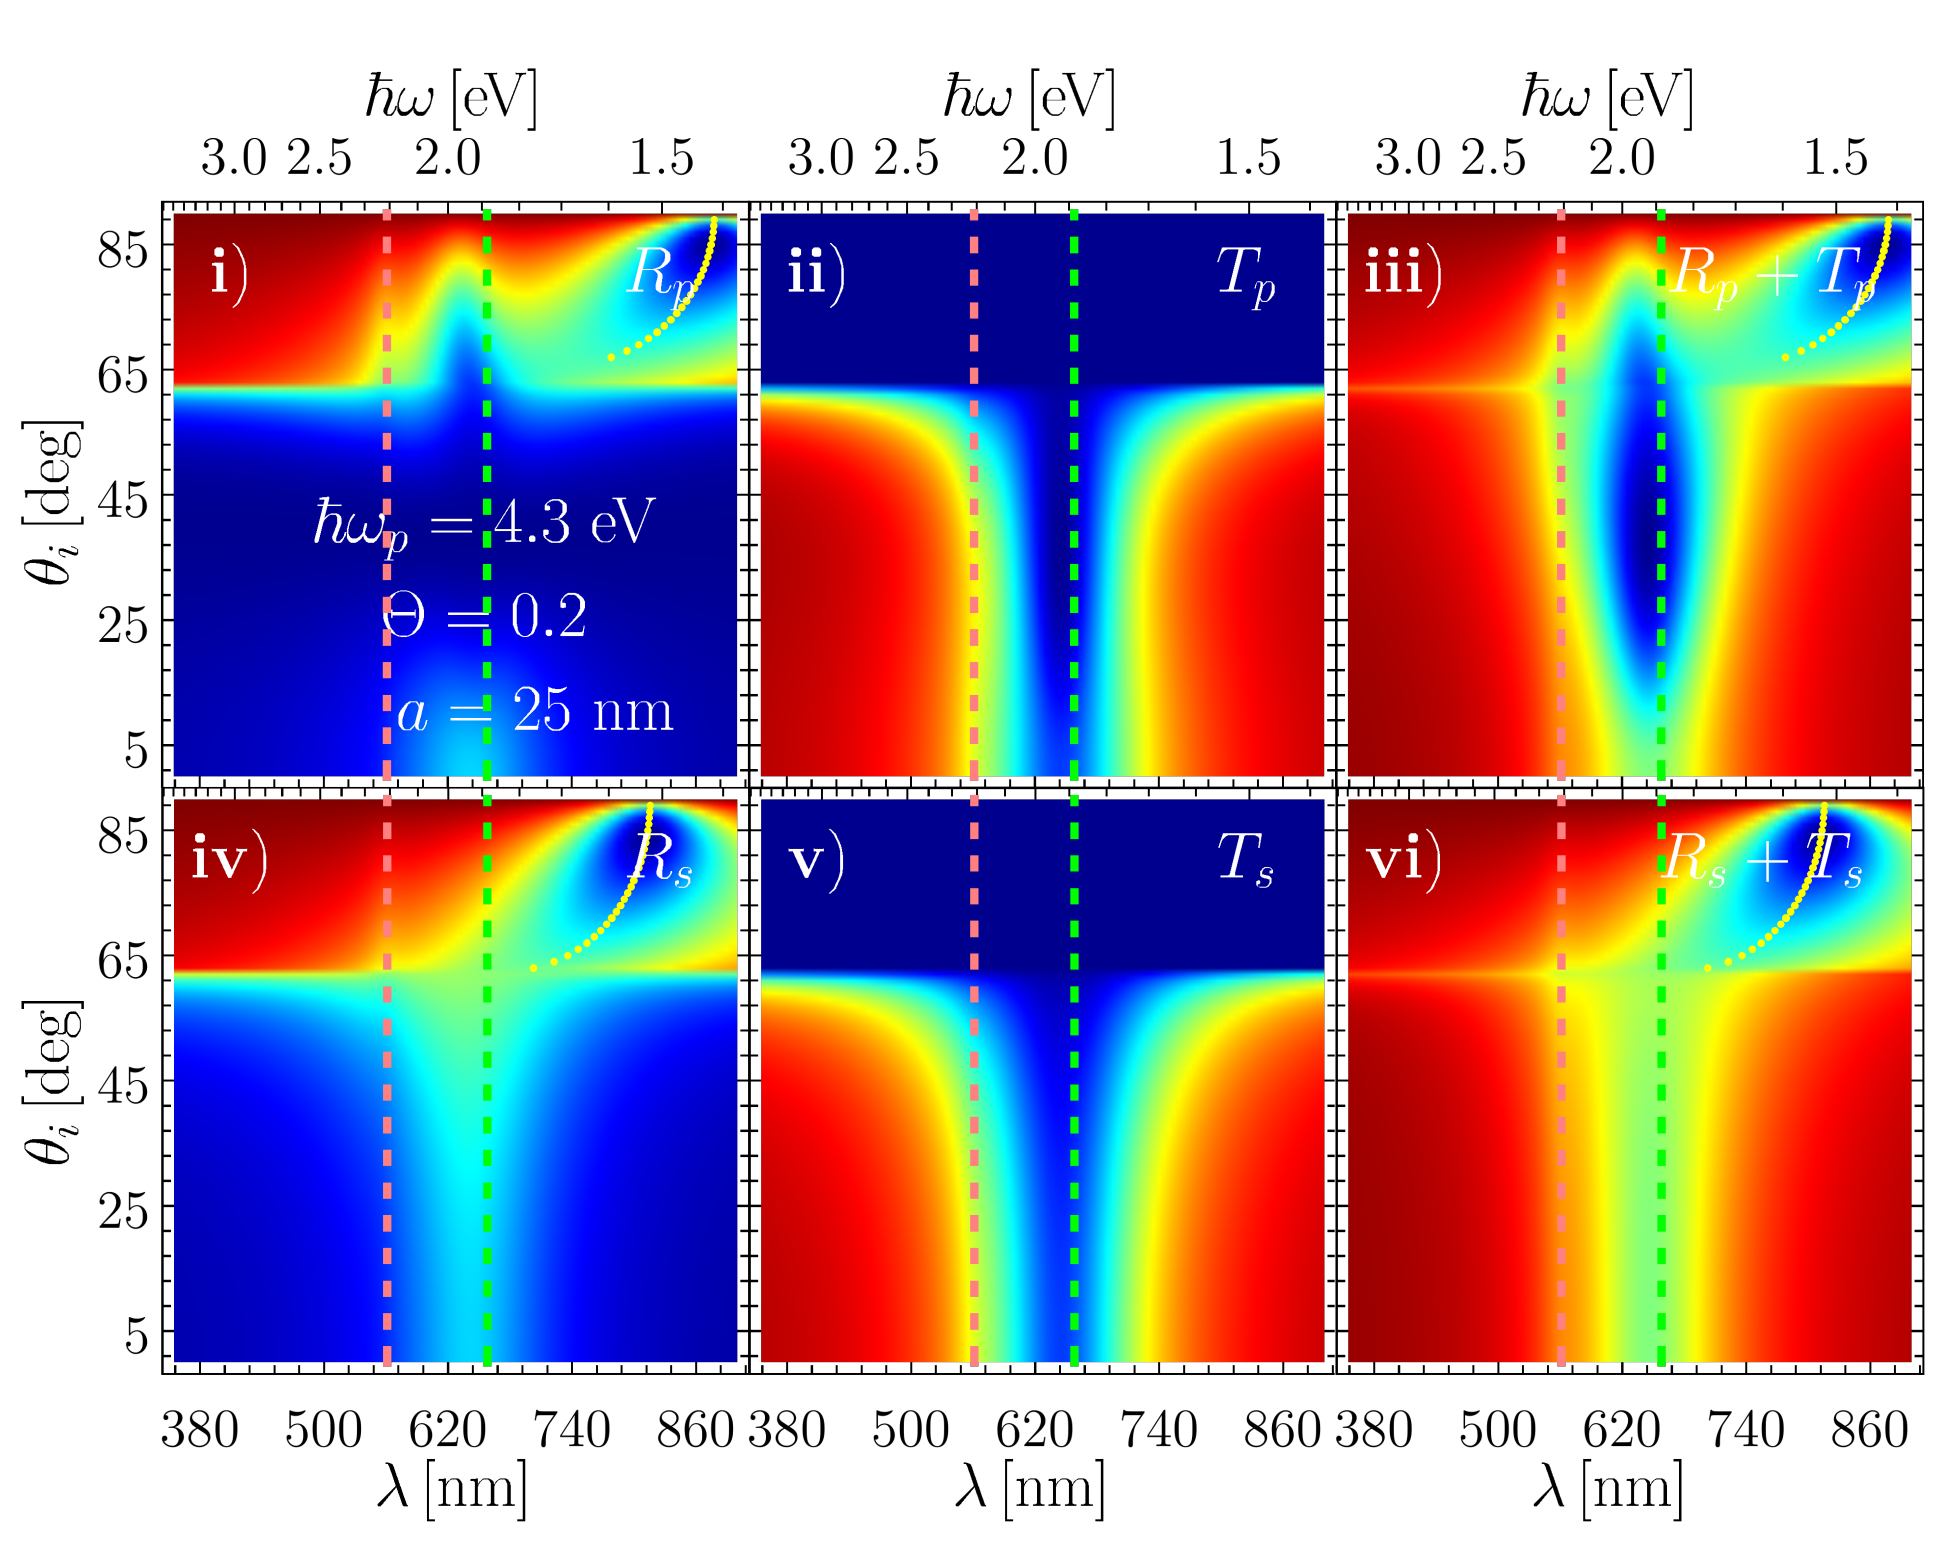
\includegraphics[width = \linewidth]{2-Resultados/figs/5-RT-Wp4-10/0-2D_Grid_1.png}};
\node[right, inner sep=0pt] (legend) at (5.6,0) {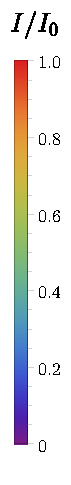
\includegraphics[scale=.975, trim={00 00 00 00}, clip]{2-Resultados/figs/0-IBar_v}};
\node[above, inner sep=0pt] (r) at (5.9,4.2) { $I/I_0$};
\end{tikzpicture}	
	\end{subfigure}\\
	\begin{subfigure}{.01\linewidth}\caption{}\label{sfig:RT-10}\vspace{6.5cm}\end{subfigure}\hspace*{-.5em}
	\begin{subfigure}{.7\linewidth}
	\begin{tikzpicture}
\node[inner sep=0pt] (graf) at (.05,0){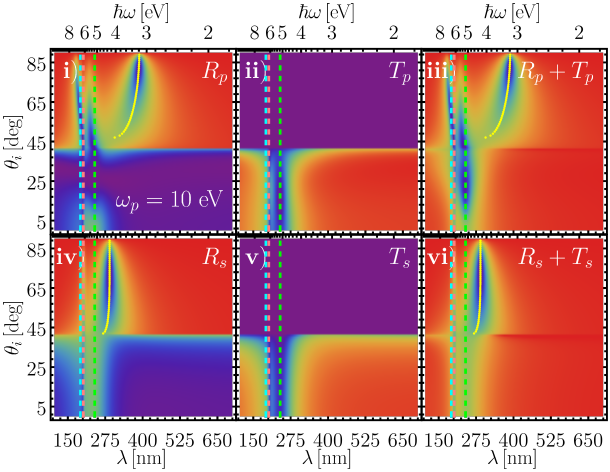
\includegraphics[width =\linewidth]{2-Resultados/figs/5-RT-Wp4-10/0-2D_Grid_2.png}};
\node[right, inner sep=0pt] (legend) at (5.6,0) {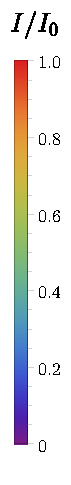
\includegraphics[scale=.96, trim={00 00 00 00}, clip]{2-Resultados/figs/0-IBar_v}};
\node[above, inner sep=0pt] (r) at (5.9,4.2) { $I/I_0$};
\end{tikzpicture}
		\end{subfigure}\vspace*{-.5em}
	\caption{Gráficas de reflectancia $R$, transmitancia $T$ y la suma de éstas $R+T$ de una monocapa en configuración ATR como función del ángulo de incidencia $\theta_i$ y de la longitud de onda $\lambda$ (escala inferior) así como de la energía del haz incidente en unidades de $\hbar\omega$ (escala superior), para una función dieléctrica tipo Drude con \textbf{a)} $\hbar\omega_p=4. 3$ eV  y  $\hbar\gamma=0. 15$ eV y \textbf{b)} $\hbar\omega_p = 10$ eV y $\hbar\gamma = 0.15$ eV.  Las gráficas   en el renglón superior [$\mathbf{i)-ii)}$]  muestran los resultados de reflectancia para  polarización \emph{p} y las del renglón inferior  [$\mathbf{iv)-vi)}$] para polarización  \emph{s}, donde se consideraron NPs de radio $a=30$ nm. Las líneas verticales punteadas verdes corresponden a la SP-SPRs dipolar ($658$ nm y $342$ nm para $\hbar\omega_p=4.3$ eV y $\hbar\omega_p = 10$ eV, respectivamente), y las rosas a la SP-SPR cuadrupolar ($561$ nm y $262$ nm para $\hbar\omega_p=4.3$ eV y $\hbar\omega_p = 10$ eV, respectivamente). Los puntos amarillos corresponden a los mínimos en $R$, y $R+T$ para ángulos mayores a $\theta_c\approx 62.5^\circ$ y longitudes de onda mayores a la SP-SPRs dipolar. }\label{fig:RT-Omegas}
	\end{figure}	

Para ambos casos analizados en la Fig. \ref{fig:RT-Omegas}, $\hbar\omega_p = 4.3$ eV y $\hbar\omega_p = 10$ eV, se observa que para valores de $\lambda$ cercanos a los de las SP-SPRs (líneas punteadas verticales) la reflectancia $R$ presenta máximos locales para ángulo de incidencia $\theta_i<\theta_c \approx 62.5^\circ$, debido al esparcimiento de luz a esa longitud de onda, y mínimos locales para $\theta_i>\theta_c$, causado por la extinción de luz (tanto esparcimiento como absorción). De forma contraria, la transmitancia $T$ es cercana a cero para todo $\theta_i$ en los valores de $\lambda$ cercanos a los de las SP-SPRs. La suma de $R$ y $T$ [en la Fig. \ref{fig:RT-Omegas}, \textbf{iii)} y \textbf{vi)}] en los valores de $\lambda$ que corresponden a las SP-SPRs, es menor a la unidad debido a que en esta región las NPs, en el límite de partícula individual, las NPs absorben más eficientemente en comparación a su esparcimiento; en particular para $\hbar\omega_p=4.3$ eV las NPS de radio $a= 30$ nm la contribución de la absorción es tres veces la del esparcimiento cuando se excita el modo dipolar [ver Fig. \ref{sfig:Qext4-30}], mientras que para $\hbar\omega_p = 10$ eV el esparcimiento es el predominante [ver Fig. \ref{sfig:Qext4-30}]. Sin embargo, las NPs no absorben en longitudes de onda mayores a la de la SP-SPR dipolar (líneas punteadas verdes) por lo que la extinción de luz en el modo colectivo (puntos amarillos en $R$ y $R+T$) se debe al esparcimiento de los campos EMs debido a la interacción de la onda evanescente que incide sobre las NPs y éstas. Dado que la transmitancia es igual a cero en los valores de $\theta_i$ y $\lambda$ correspondientes al presunto modo colectivo, el esparcimiento de luz no ocurre en la dirección transmitida coherente, como tampoco a la reflejada, por lo que se le atribuye el comportamiento de un modo guiado.

El estudio de la excitación distinta de las SP-SPRs presente en los cálculos de la reflectancia de una monocapa de NPs esféricas e idénticas, permite catalogarlo como un modo colectivo dado que su respuesta es más apreciable al aumentar la fracción de cubierta $\Theta$ y el radio $a$ de las NPs. Asimismo, al analizar la la extinción de luz  en los cálculos de $R$ y $T$, es posible catalogar a la excitación atípica presente en la monocapa como un modo colectivo y guiado puesto que se presenta a longitudes de onda en donde las NPs no absorben y el esparcimiento de luz no corresponde a la componente coherente y, por hipótesis en la construcción del CSM, la componente difusa es despreciable respecto a ésta. Tras la caracterización de la excitación atípica como un modo guiado y colectivo, que es sintonizable según los parámetros de la monocapa, empleando el modelo de Drude-Sommerfeld para la función dieléctrica de las NPs, se analiza si esta excitación colectiva es apreciable en materiales más realistas. En la siguiente sección se presentan los resultados de la respuesta EM de una monocapa conformado por NPs de oro y plata, es decir, empleando como función dieléctrica de las NPs la corrección por tamaño de los datos experimentales para el oro y plata en bulto de \cite{johnson1972constants}.

